%&"..\virtual"

\begin{document}
    \title{DPDK}
    \maketitle
    \tableofcontents
    \section{要求}

    DPDK performance test:

    \begin{enumerate}[(1)]
        \item Create two virtual machines on KVM.
        \item Compile and install DPDK library on each virtual machine.
        \item Compile and run DPDK sample application l2fwd on VM2, then compile and run pktgen-dpdk on VM1.  pkgen-dpdk will record the size of the packages VM1 sends and the amount of packages received from VM2,  while l2fwd just send back the packages it received from VM1.
        \item Evaluate DPDK's performance of L2 forwarding.
    \end{enumerate}

    \section{编译安装 DPDK}\label{sec:compile}

    按照官方文档\cite{dpdk}编译 DPDK,如图 \ref{fig:meson} 、\ref{fig:ninja}、 \ref{fig:ninjainstall} 所示。

    \code[language=bash]{INSTALL.sh}

    \begin{figure}[H]
        \centering
        \begin{minipage}{0.48\textwidth}
            \centering
            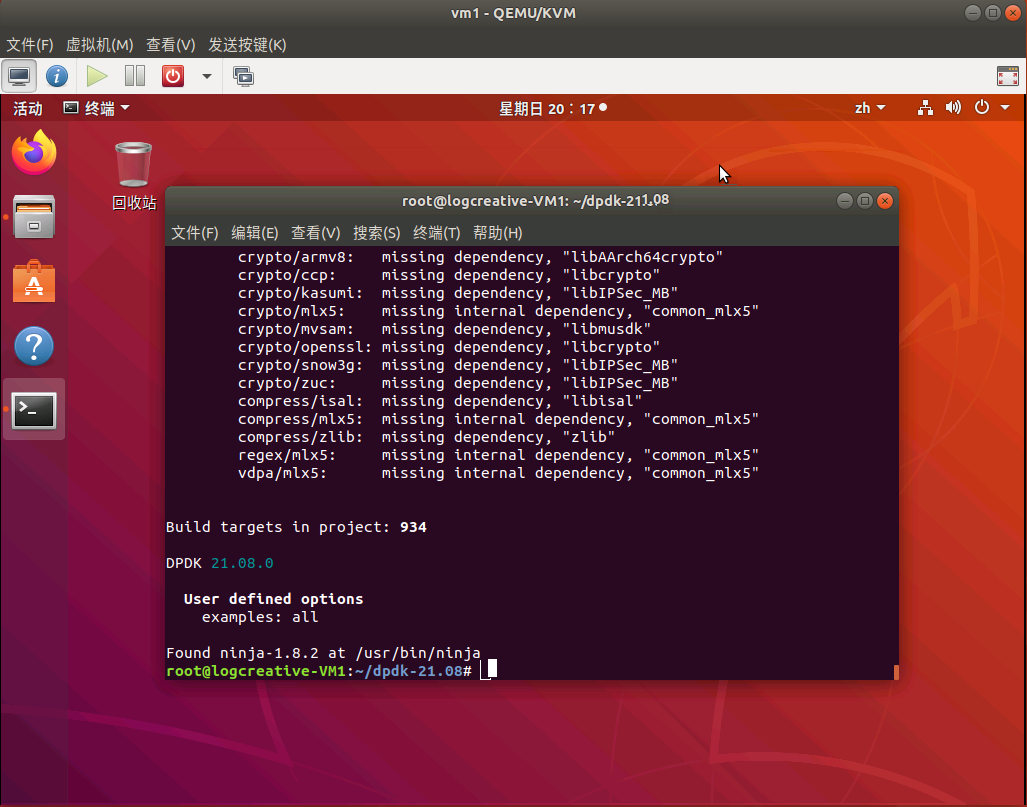
\includegraphics[width=\linewidth]{meson}
            \caption{meson 配置}\label{fig:meson}
        \end{minipage}
        \begin{minipage}{0.48\textwidth}
            \centering
            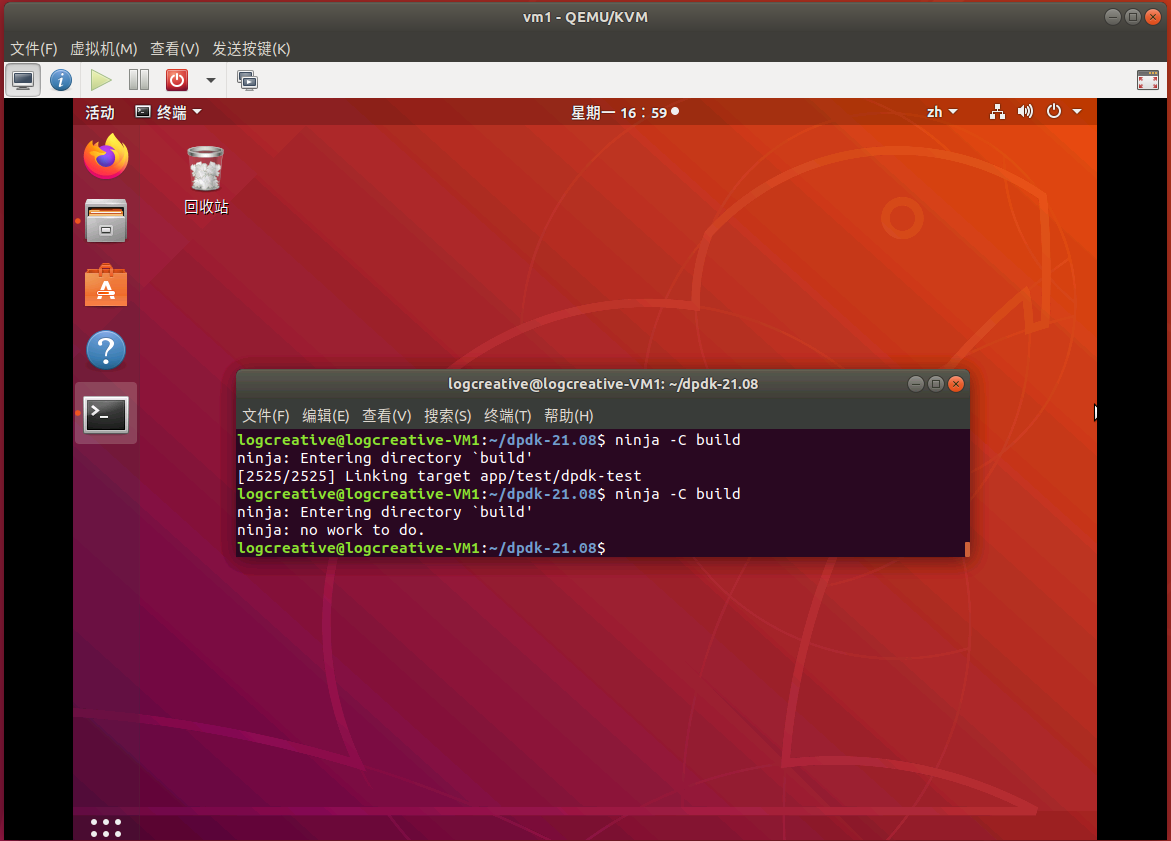
\includegraphics[width=\linewidth]{ninja}
            \caption{ninja 编译}\label{fig:ninja}
        \end{minipage}
    \end{figure}

    之后对该虚拟机进行克隆,得到另一个已经安装 DPDK 的虚拟机,如图 \ref{fig:vmclone} 所示。

    \begin{figure}[H]
        \centering
        \begin{minipage}{0.45\textwidth}
            \centering
            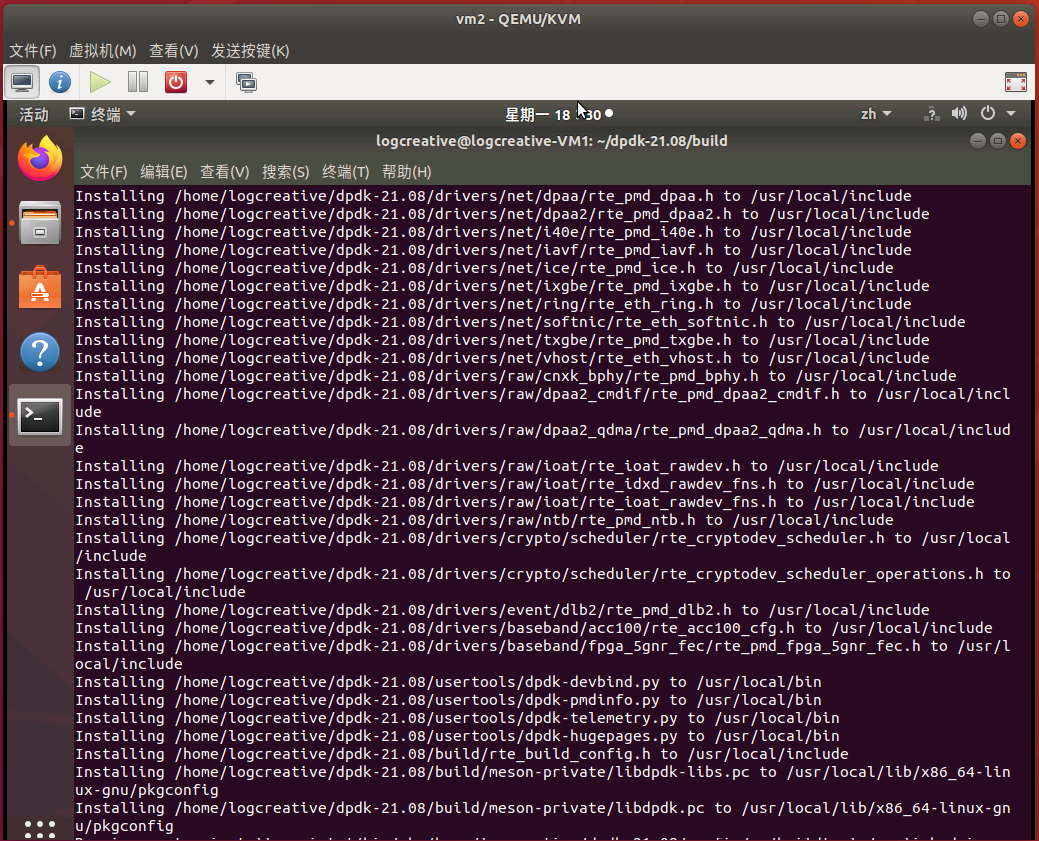
\includegraphics[width=\linewidth]{ninjainstall}
            \caption{ninja 安装}\label{fig:ninjainstall}
        \end{minipage}
        \begin{minipage}{0.3\textwidth}
            \centering
            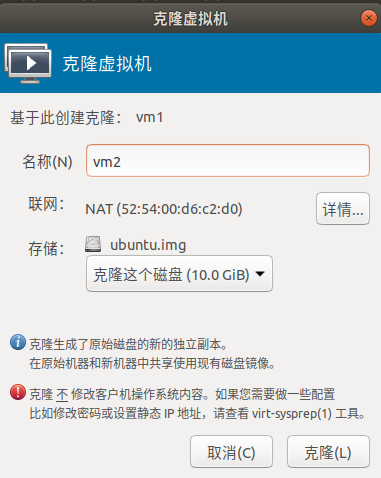
\includegraphics[width=\linewidth]{vmclone}
            \caption{克隆虚拟机}\label{fig:vmclone}
        \end{minipage}
    \end{figure}

    \section{配置网卡}

    通过 virt-manager 设置两个虚拟机为两个网卡的 NAT 网络连接(如图 \ref{fig:nat}),然后需要在两个虚拟机上加载 \verb"uio_pci_generic" 驱动\cite{openuio},然后绑定在 DPDK 上\cite{bind}(如图 \ref{fig:bindcard})。

    \begin{figure}[H]
        \centering
        \begin{minipage}{0.48\textwidth}
            \centering
            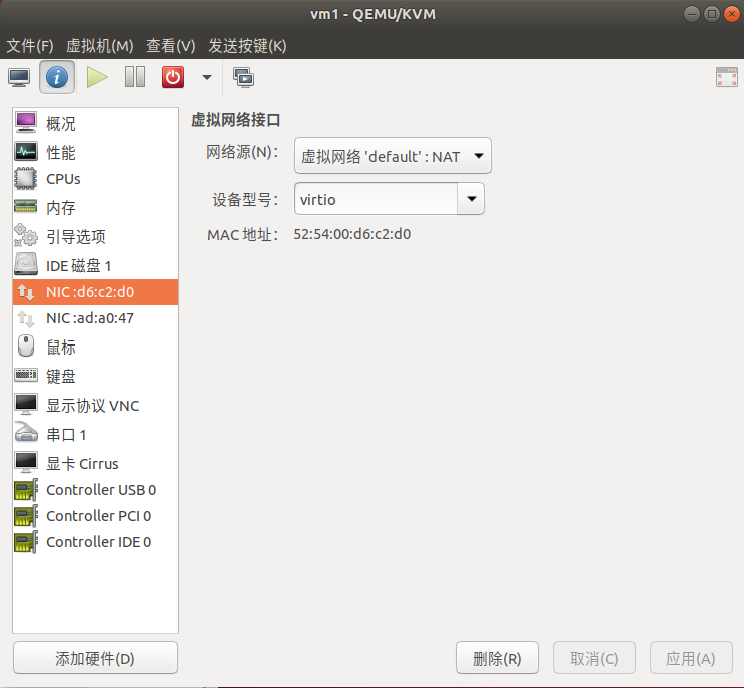
\includegraphics[width=\linewidth]{nat}
            \caption{NAT 设置}\label{fig:nat}
        \end{minipage}
        \begin{minipage}{0.48\textwidth}
            \centering
            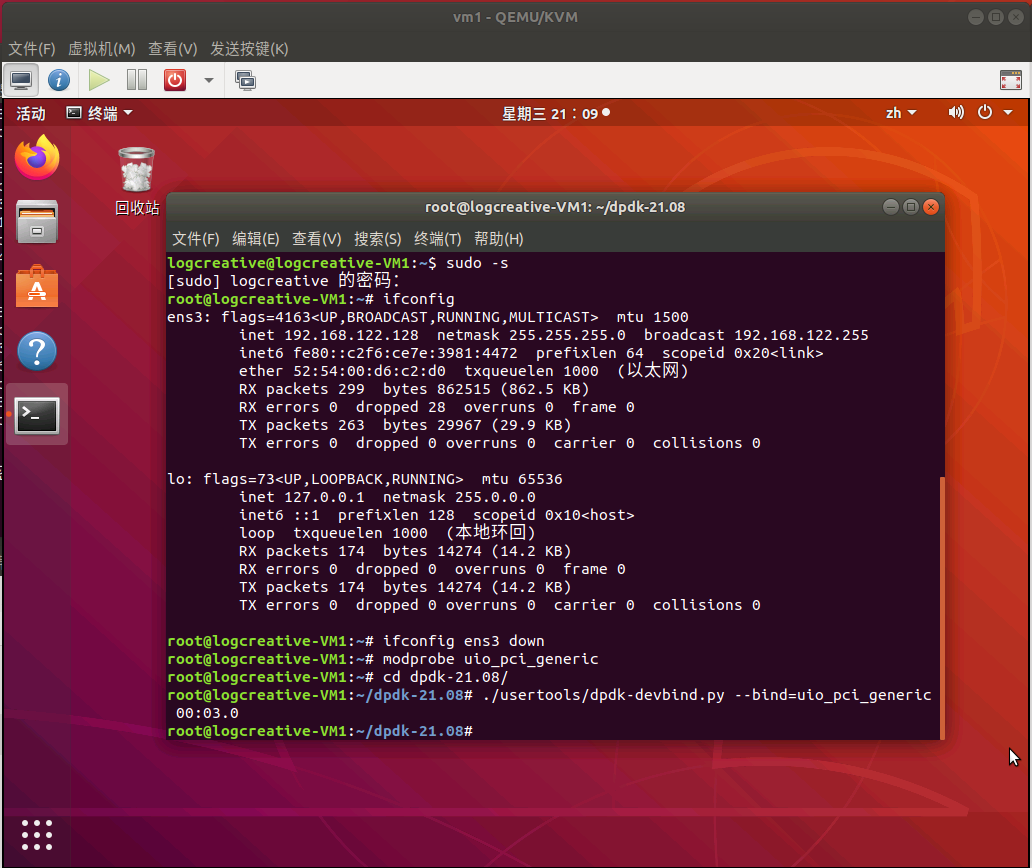
\includegraphics[width=\linewidth]{bindcard}
            \caption{DPDK 绑卡}\label{fig:bindcard}
        \end{minipage}
    \end{figure}

    \code[language=bash]{nic.sh}

    \section{编译 l2fwd pktgen}

    这一步在上一步配置完成后进行,需要用到已经配置好的 DPDK 库。在 VM2 上编译 l2fwd,如图 \ref{fig:makel2fwd}。编译前需要修改 l2fwd 的 \verb"main.c" 其中一行,关闭混杂模式\cite{dpdkl2},也就是注释下面这一行(不同的版本可能行号不同)。

    \codeseg[language=c]{../dpdk/examples/l2fwd/main.c}{883}{883}

    \code[language=bash]{l2fwd.sh}

    \begin{figure}[H]
        \centering
        \begin{minipage}{0.48\textwidth}
            \centering
            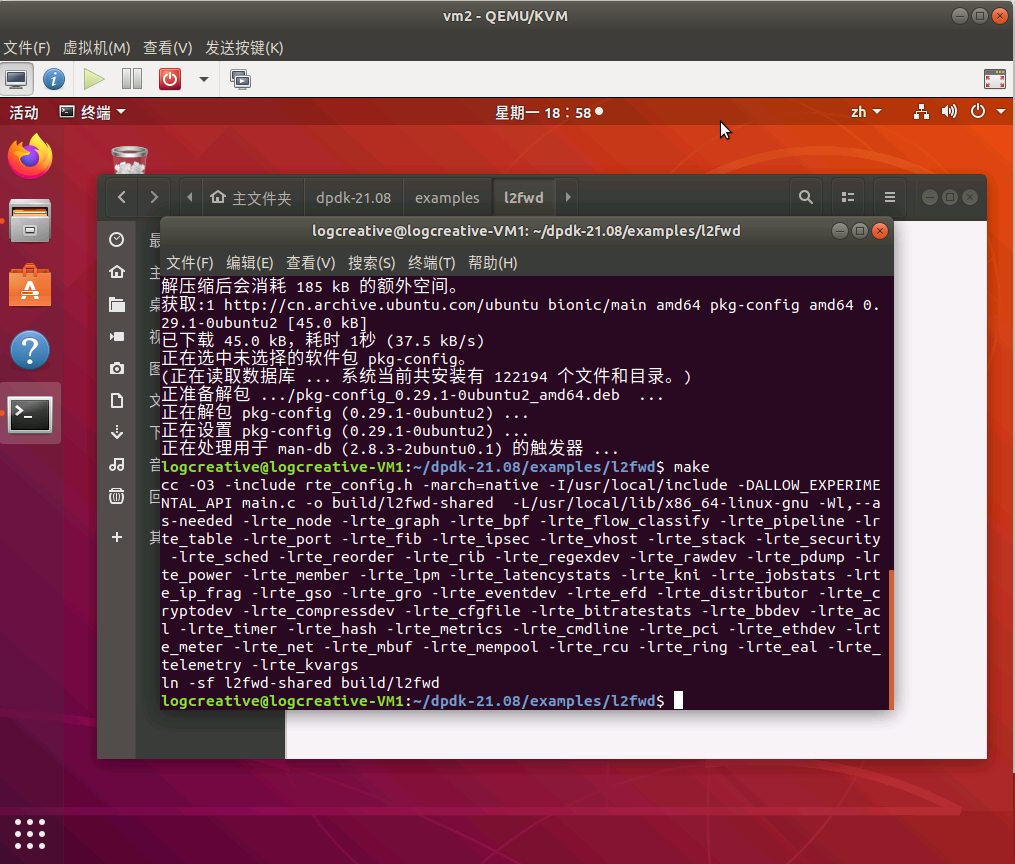
\includegraphics[width=\linewidth]{makel2fwd}
            \caption{l2fwd 编译}\label{fig:makel2fwd}
        \end{minipage}
        \begin{minipage}{0.48\textwidth}
            \centering
            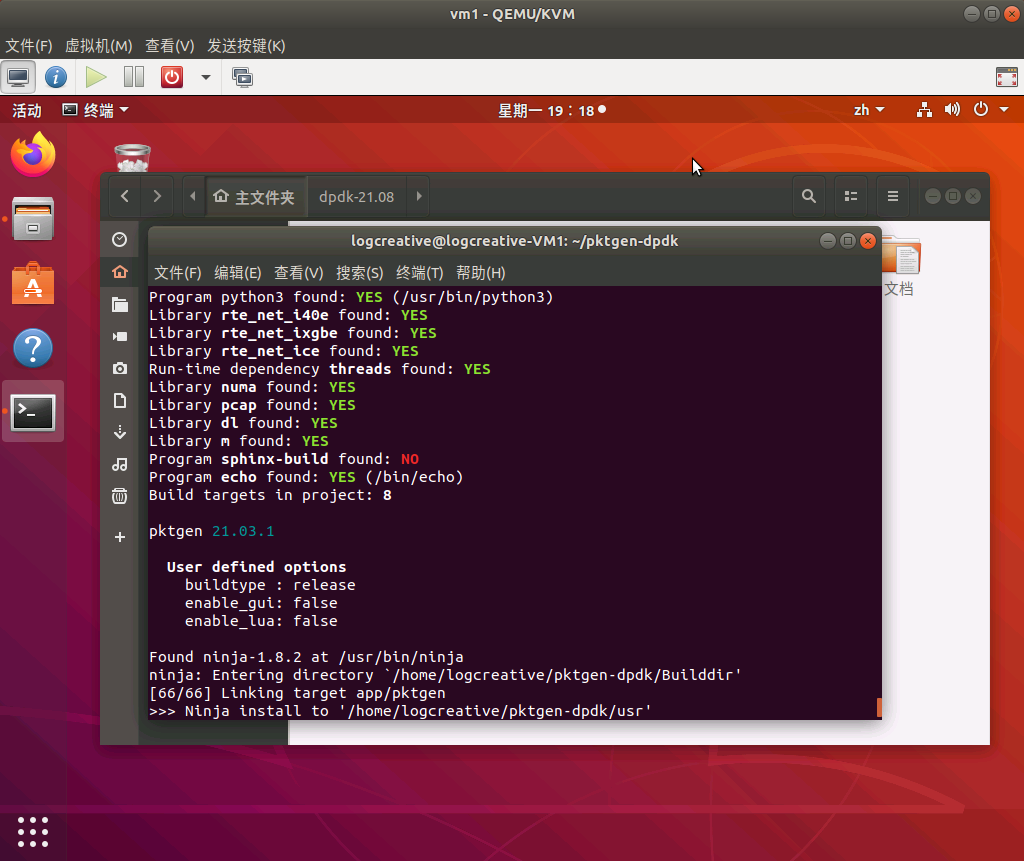
\includegraphics[width=\linewidth]{makepktgen}
            \caption{pktgen 编译}\label{fig:makepktgen}
        \end{minipage}
    \end{figure}

    在 VM1 上编译 pktgen,如图 \ref{fig:makepktgen}。

    \code[language=bash]{pktgen.sh}

    \section{运行测试}

    同时打开两个虚拟机\footnote{请不要分配超过限制的 CPU 数量,否则会闪退。这里为每一个虚拟机分配了 2 个核。}。启动测试的方法是在两个虚拟机上分别运行对应的部分\cite{l2fwduse},配置完成后如图 \ref{fig:basicconf} 所示。

    如果运行失败,需要重新分配 Hugepages(可能已经用光了),方法见第 \ref{sec:compile} 节。注意在运行 l2fwd 时加了 \verb"--no-mac-updating" 参数,因为不需要发送过多的 ARP 包污染计数\cite{dpdkl2}。

    在 pktgen 的 CLI 中更改 count 的数目,以检测瞬时的包接收性能。

    \code[language=bash]{test.sh}

    这样得到的发包拓扑如图 \ref{fig:topo} 所示。

    \begin{figure}[H]
        \centering
        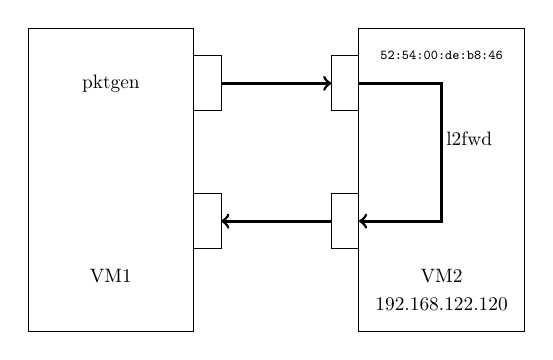
\begin{tikzpicture}[scale=0.7,every node/.style={scale=0.7}]

\draw  (-3,2.5) rectangle (0,-3);
\draw  (3,2.5) rectangle (6,-3);
\draw  (0,2) rectangle (0.5,1);
\draw  (2.5,2) rectangle (3,1);
\draw  (0,-0.5) rectangle (0.5,-1.5);
\draw  (2.5,-0.5) rectangle (3,-1.5);
\draw[->,line width=1pt] (0.5,1.5) -- (2.5,1.5);
\draw[->,line width=1pt] (2.5,-1) -- (0.5,-1);
\draw[->,line width=1pt] (3,1.5) -- (4.5,1.5) -- (4.5,-1) -- (3,-1);
\node at (4.5,-2) {VM2};
\node at (-1.5,-2) {VM1};
\node at (-1.5,1.5) {pktgen};
\node at (5,0.5) {l2fwd};
\node[font=\ttfamily\scriptsize] at (4.5,2) {52:54:00:de:b8:46};
\node at (4.5,-2.5) {192.168.122.120};
\end{tikzpicture}
        \caption{发包拓扑}\label{fig:topo}
    \end{figure}

    \begin{figure}[H]
        \centering
        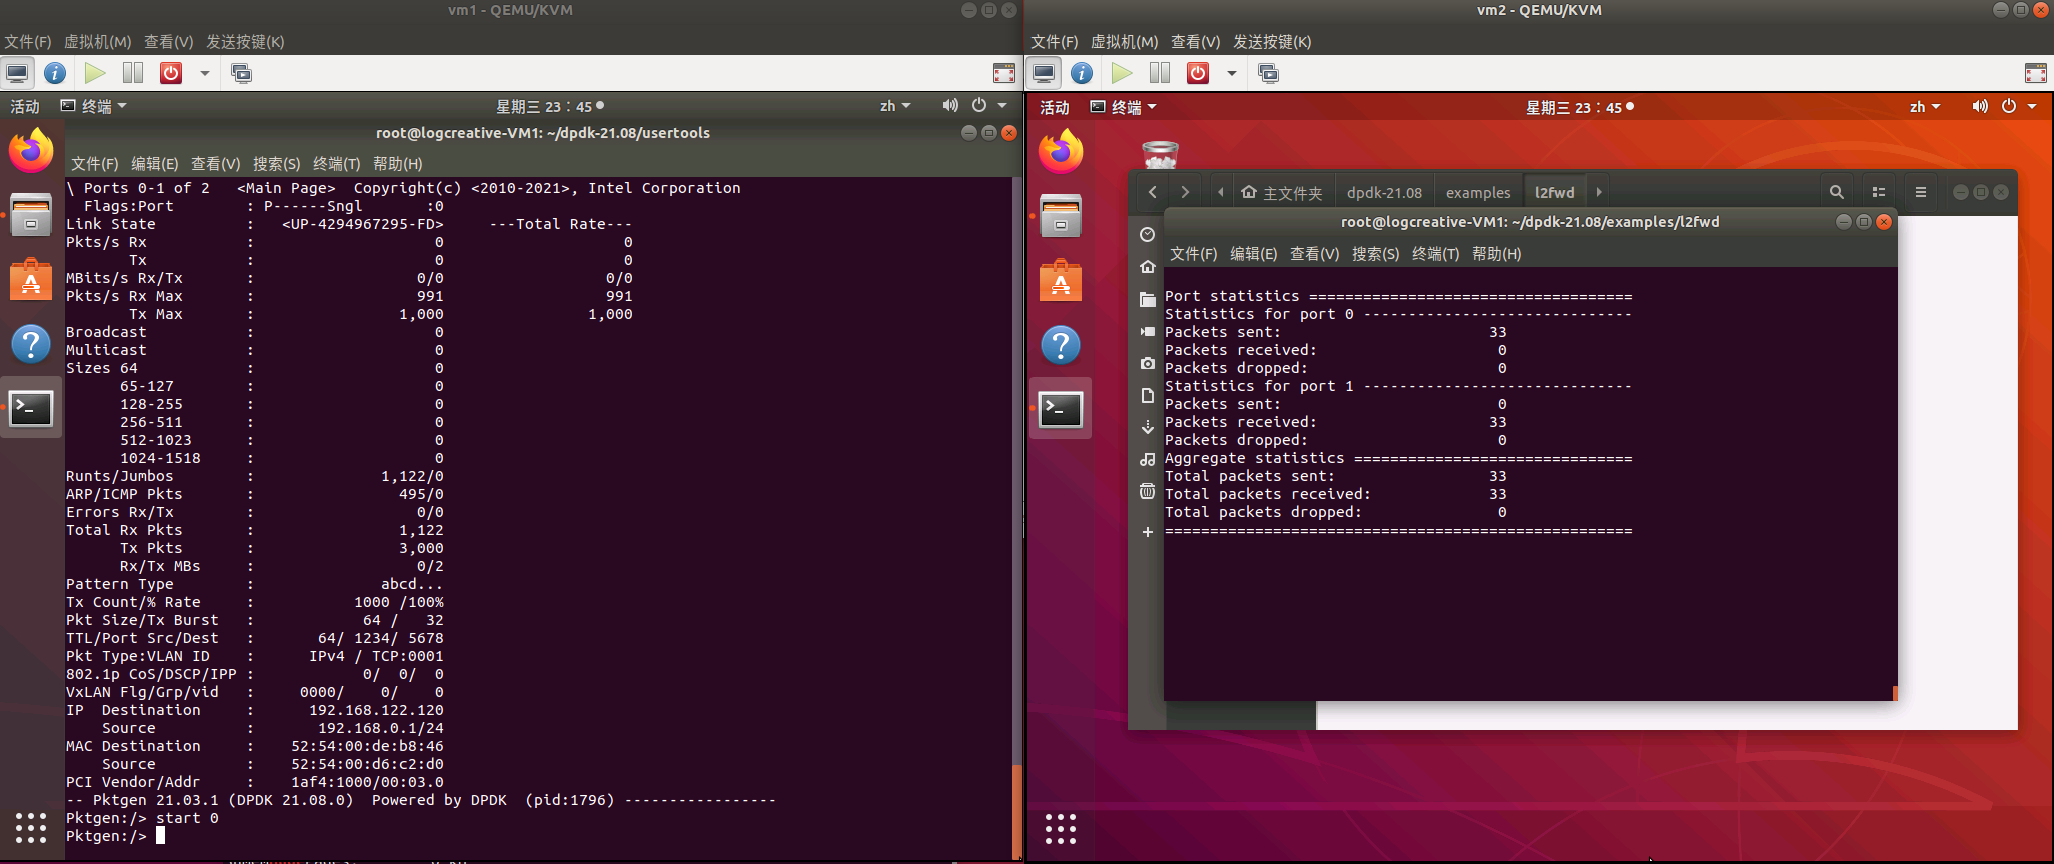
\includegraphics[width=\linewidth]{basicconf}
        \caption{两个虚拟机的配置}\label{fig:basicconf}
    \end{figure}

    \section{评估}

    \begin{figure}[H]
        \centering
        \begin{minipage}{0.48\textwidth}
            \centering
            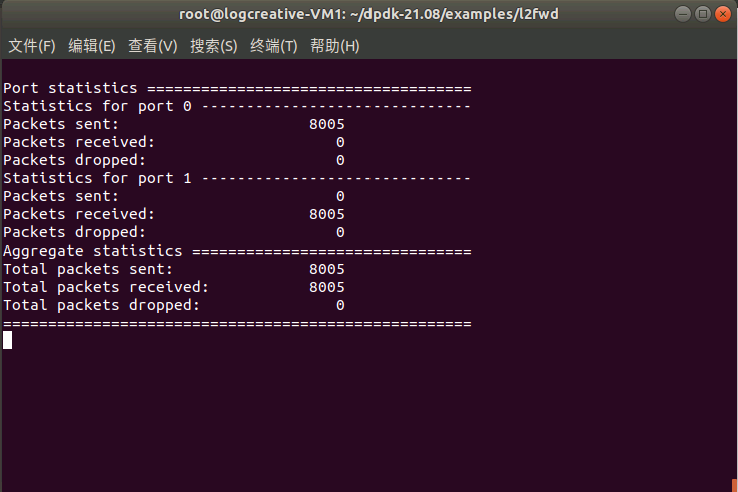
\includegraphics[width=\linewidth]{8000}
            \caption{发包数 8000}\label{fig:8000}
        \end{minipage}
        \begin{minipage}{0.48\textwidth}
            \centering
            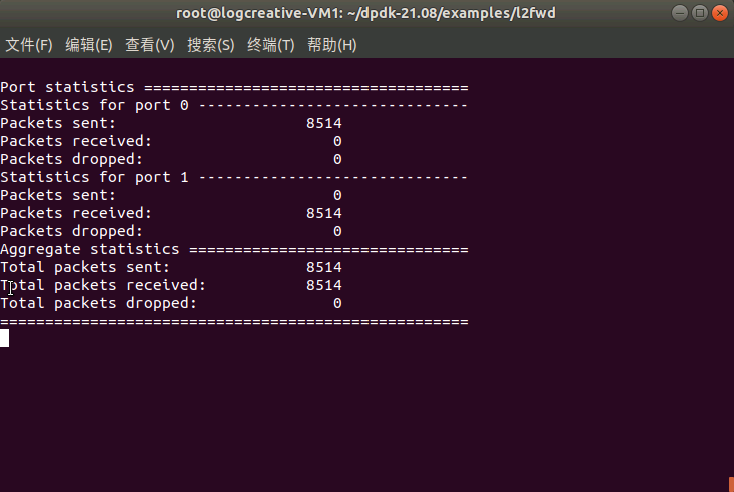
\includegraphics[width=\linewidth]{10000}
            \caption{发包数 10000}\label{fig:10000}
        \end{minipage}
    \end{figure}

    如图 \ref{fig:8000} 所示,在瞬时发包数为 8000 时还是不丢包的。而如图 \ref{fig:10000} 所示,在瞬时发包数为 10000 时丢了一部分包(15\%),也就是性能瓶颈大概在 8500 个包左右,性能还是很可观的,约等于几千个程序同时服务。

    于此形成对照的是使用下面的脚本(使用原生的 pktgen\cite{pktgen}),10000 发包数丢失 40\% 左右的包。

    \code[language=bash]{comparetest.sh}

    所以 DPDK 运行在操作系统的 User Space,利用自身提供的数据面库进行收发包处理,绕过了 Linux 内核态协议栈\cite{dpdkinfo},可以大幅提高包的转发效率。

    \section*{运行环境}

    附运行环境如表 \ref{tab:env} 所示。

    \begin{table}[H]
    \centering
    \caption{运行环境}\label{tab:env}
    \begin{tabular}{ll}
        \toprule
        系统 & Ubuntu 18.04 \\
        核心数 & 2核4逻辑核 \\
        虚拟机分配逻辑核 & 2 \\
        虚拟机内存 & 1024MB \\
        虚拟机网卡 & virtio \\
        DPDK 版本 & 21.08 \\
        pktgen 版本 & 20.02 \\ 
        \bottomrule
    \end{tabular}
    \end{table}

    \bibliography{ref}

\end{document}